\chapter{Stable Distribution}

\section{Stable Distribution}

\subsection{Definition of stable distribution}

\begin{definition}[stable distribution\index{stable distribution}, strictly stable distribution\index{strictly stable distribution}]\label{def:stable distribution_1}
Let $X,X_1,\dots, X_n$ be independent and identically distributed random variables with non-degenerate distribution $F$. Then the distribution of $F$ is stable if for each $n$ there exist constants $a_n>0$ and $b_n \in \R$ such that
\be
S_n := X_1 + \dots + X_n \sim a_n X + b_n 
\ee
where $\sim$ means two random variables have the same distribution. $F$ is strictly stable if 
\be
S_n := X_1 + \dots + X_n \sim a_n X.
\ee

Note that $a_n$ and $b_n$ are the norming constants.% and $b_n$ is centering constant.
\end{definition}

\begin{remark}
The stable distribution family is also sometimes referred to as the \levy\ alpha-stable distribution, after Paul \levy, the first mathematician to have studied it.
\end{remark}

\begin{proposition}\label{pro:stable distribution_2}
If $X,X_1,X_2$ are independent and identically distributed with distribution function $F$. Then $F$ is stable if and only if for arbitrary constants $a_1,a_2$ there exist constants $a,b$ such that 
\be
a_1 X_1 + a_2 X_2 \sim a X + b.
\ee 
\end{proposition}

\begin{theorem}\label{thm:stable_distribution_continuity}
Every stable distribution is continuous.
\end{theorem}

\begin{proof}[\bf Proof]
\footnote{see Feller book, \cite{Feller_1970}.p215}
\end{proof}

\begin{theorem}[characteristic exponent of distribution]\label{thm:characteristic_exponent_distribution}
Let non-degenerate distribution $F$ be stable distribution denoted by
\be
S_n := X_1 + \dots + X_n \sim a_n X + b_n.
\ee

Then the norming constants are of the form $a_n =n^{1/\alpha}$ with $0<\alpha \leq 2$. The constant $\alpha$ is called the characteristic exponent of distribution $F$\index{characteristic exponent!distribution}.
\end{theorem}

\begin{remark}
The proof is due to \cite{Feller_1970,Uchaikin_Zolotarev_1999}.
\end{remark}

\begin{proof}[\bf Proof]
The argument is greatly simplified by symmetrization. If $F$ is stable so is the distribution $F^0$ of $X_1-X_2$ and the norming constants $a_n$ are the same. It suffices therefore to prove the assertion for a symmetric stable $F$.

We start from the simple remark that $S_{m+n}$ is the sum of the independent variables $S_m$ and $S_{m+n}-S_m$ distributed, respectively, as $a_mX$ and $a_n X$.\footnote{$S_n$ the summation of $n$ independent and identically distributed $X_i$ with distribution $F$.} Thus for symmetric stable distributions 
\be
a_{m+n}X \sim a_m X_1 + a_n X_2.\qquad (*)
\ee

Similarly, the sum $S_{mn}$ can be broken up into $n$ independent blocks of $m$ terms each, whence $a_{mn} = a_ma_n$ for all $m$ and $n$. Then for the form $n = r^i$ we conclude by induction that $a_n = a_r^i$. Furthermore, for $n = r^i$,
\be
a_n = a_r^i = a_r^{i\log r/\log r} = a_r^{\log n /\log r} \ \ra\ \log a_n = \frac{\log n}{\log r}\log a_r = \log n^{\frac{\log a_r}{\log r}}\ \ra\ a_n = n^{1/\alpha_r}
\ee
where $\alpha_r := \log r/\log a_r$. That means for any $n=r^i$, their norming constants are of the form of $n^{1/\alpha_r}$.

Next put $u = m+n$ and by the symmetry of $a_{m+n}X$ we have for $t>0$,
\beast
\pro\bb{X>t} & = & \pro\bb{\frac{a_m}{a_u} X_1 + \frac{a_n}{a_u} X_2>t} = \pro\bb{\frac{a_m}{a_u}  X_1  >t - \frac{a_n}{a_u} X_2} \\
& = & \pro\bb{\frac{a_m}{a_u}  X_1  >t - \frac{a_n}{a_u} X_2, X_1\geq 0} + \pro\bb{\frac{a_m}{a_u}  X_1  >t - \frac{a_n}{a_u} X_2, X_1\leq   0} \\
& = & \pro\bb{X_1\geq 0}\pro\bb{\left.\frac{a_m}{a_u}  X_1  >t - \frac{a_n}{a_u} X_2,\right| X_1\geq 0} + \pro\bb{X_1\geq 0} \pro\bb{\left.\frac{a_m}{a_u}  X_1  >t - \frac{a_n}{a_u} X_2,\right| X_1\leq   0} \\
& \geq & \frac 12 \pro\bb{0  >t - \frac{a_n}{a_u} X_2} = \frac 12 \pro\bb{X_2  >\frac{a_u }{a_n}t }.\qquad (\dag)
\eeast

Note that $F$ is continuous at 0 since $F$ is symmetric (and thus right continuous and left continuous). If $a_n/a_u$ is not bounded, we have $\frac{a_u }{a_n} = 0$, thus by ($\dag$) for any $t>0$, 
\be
\pro\bb{X>t} \geq \frac 12 \pro\bb{X_2 > 0} > 0 \ \ra\ \pro(X= \infty) >0
\ee
which is a contradiction. Thus for any $n$ and all $u>n$ the ratios $a_n/a_u$ is bounded ($\ddag$). If $u=n^i$ with $i\geq 2$, we have that 
\be
\frac{a_n}{a_u} = \frac{n^{1/\alpha_n}}{n^{i/\alpha_n}} = n^{(1-i)/\alpha_n}.
\ee

Thus, $\alpha_n >0$, otherwise the ratio is unbounded when $i \to \infty$. 
%
%\be
%\pro\bb{X>t} = \frac 12\pro\bb{\abs{X} >t} = \frac 12 \pro\bb{\abs{\frac{a_m}{a_u} X_1 + \frac{a_n}{a_u} X_2} >t} = \frac 12 \pro\bb{\abs{\frac{a_m}{a_u} X_1 - \frac{a_n}{a_u} X_2} >t}
%\ee
%
%Since $\bra{\abs{\frac{a_m}{a_u} X_1 - \frac{a_n}{a_u} X_2} >t} \subseteq \bb{\bra{\abs{X_1}\leq  \frac{a_m}{a_u} t} \cap \bra{\abs{X_2}\leq \frac{a_n}{a_u} t} }^c = \bra{\abs{X_1} >  \frac{a_m}{a_u} t} \cup \bra{\abs{X_2} > \frac{a_n}{a_u} t} $

%Then $\alpha_r >0$ for $n = r^i$
%
%if $\alpha_p < 0$
%
%Then $\alpha_{rk} > 0$ then for all composite number

Now we want to show that for any integer $n$ there exists a unique $\alpha$ such that $a_n = n^{1/\alpha}$. Since $a_{mn} = a_ma_n$ for any $m,n$, it suffices to show that if $a_n = n^{1/\alpha_r}$ and $a_m = m^{1/\alpha_t}$, then $\alpha_r = \alpha_t$. For each $m = t^j$ there exists an $n = r^i$ such that $n< m\leq rn$ with $a_n = n^{1/\alpha_r}$ and $a_m = m^{1/\alpha_t}$. Then
\be
a_m = m^{1/\alpha_t} \leq \bb{rn}^{1/\alpha_t} = r^{1/\alpha_t} a_n^{\alpha_r/\alpha_t}.
\ee

If $\alpha_t > \alpha_r$,
\be
\frac{a_m}{a_n} \leq r^{1/\alpha_t} a_n^{\alpha_r/\alpha_t-1} = r^{1/\alpha_t} n^{\frac{\alpha_r-\alpha_t}{\alpha_r\alpha_t}} \to 0 
\ee
as $n\to\infty$. This implies that $a_n/a_m$ is unbounded which is contradiction with ($\ddag$). Therefore, $\alpha_t \leq \alpha_r$. Interchanging the role of $r$ and $t$, we find similarly that $\alpha_t \geq \alpha_r$ and hence $\alpha_t = \alpha_r$. 


To prove that $\alpha \leq 2$ we remark that the normal distribution is stable with $\alpha =2$.\footnote{details needed.} Moreover, if the random variable has finite variance we have %For it ($*$) reduces to the addition rule for variance, and the latter implies that any stable distribution with finite variances necessarily corresponds to $\alpha = 2$.
\be
n^{2/\alpha} \var X = a_n^2 \var X = \var\bb{a_{n}X} = \var\bb{\sum^n_{i=1}X_i} = n \var X_i \ \ra\ \alpha = 2.
\ee

To conclude the proof it suffices therefore to show that any stable distribution with $\alpha>2$ would have a finite variance. For symmetric distributions $S_n := X_1 + \dots + X_n \sim a_n X + b_n $ holds with $b_n = 0$, and hence we can choose $t$ such that for all $n$,
\be
\pro\bb{\abs{S_n} > ta_n} = \pro\bb{\abs{X} >t} < \frac 14.
\ee

Then by Lemma \ref{lem:distribution_symmetrization_inequalities}, we have 
\be
\frac 14 > \pro\bb{\abs{S_n} > ta_n} \geq \frac 12 \bb{1 - e^{-n\bb{1-F(ta_n) + F(-ta_n)}}} \ \ra\ 1 - e^{-2n\bb{1-F(ta_n) }} \leq \frac 12 \ \ra\ n\bb{1-F(ta_n)} \leq \frac 12 \ln 2 \nonumber
\ee
since $F$ is symmetric. Then we can see that $(n+1)\bb{1-F(ta_n)}$ is bounded by $\frac 12 \ln 2 + 1$. Then if $ta_{k}< x\leq ta_{k+1}$ where $k=1,2,\dots$, we have
\beast
x^\alpha \bb{1-F(x)} & = & \bb{ta_{k+1}}^{\alpha} \bb{1-F(ta_k)} = \bb{t\bb{k+1}^{1/\alpha}}^{\alpha} \bb{1-F(ta_k)} \\
& = & t^\alpha (k+1)\bb{1-F(ta_k)} \leq t^\alpha \bb{\frac 12 \ln 2 + 1} := M
\eeast

Therefore, $x^\alpha \bb{1-F(x)}$ is bounded by $M$ for all $x>t$. Assume $t\in \left( 2^{n-1}, 2^{n}\right]$ where $n$ is an integer. Then
\be
2^{\alpha k}\bb{1-F\bb{2^{k}}} \leq M \ \ra\  \bb{1-F\bb{2^{k}}} \leq M2^{-\alpha k}
\ee
and thus
\beast
\var X & = & \E X^2 \leq t^2 \pro\bb{X\leq t} + \sum^\infty_{k=n-1}\int^{2^{k+1}}_{2^k} x^2 dF(x) \leq t^2 + \sum^\infty_{k=n-1} 2^{2(k+1)} \int^{2^{k+1}}_{2^k} dF(x) \\
& \leq & t^2 + 2^{2n} + \sum^\infty_{k=n-1} 2^{2(k+1)} \bb{1-F\bb{2^{k}}}  \leq t^2 + 2^{2n} + 4M \sum^\infty_{k=n-1} 2^{(2-\alpha)k} 
\eeast
which is finite as the infinite summation converges ($\alpha >2$).
\end{proof}

\begin{theorem}
If $F$ is stable with an exponent $\alpha \neq 1$, then centering constant $c$ may be chosen so that $F(x+c)$ is strictly stable.
\end{theorem}

\begin{proof}[\bf Proof]
$S_{mn}$ is the sum of $m$ independent variables each distributed as $a_n X + b_n$. Accrodingly,
\be
S_{mn} \sim a_nS_m + mb_n \sim a_na_m X + a_nb_m + mb_n.
\ee

Since $m$ and $n$ play the same role this means that we have identically
\be
(a_n - n)b_m  = (a_m - m)b_n.
\ee

When $\alpha =1$ this statement is empty, but when $\alpha \neq 1$ it implies that $b_n = -c(a_n - n)$ for all $n$. Then by the definition we have that the sum $S_n'$ of $n$ varaibles distributed as $X' := X-c$ satisfies the condition $S'_n \sim a_n X'$. That is,
\be
S'_n = \sum^n_{i=1}X_i - cn  \sim a_n X + b_n - cn = a_n (X-c) + b_n + c(a_n-n) = a_n(X-c) = a_n X'.
\ee
\end{proof} 

Similarly, we have the following proposition.

\begin{proposition}
If $F$ is strictly stable with exponent $\alpha$ then for all $s,t>0$ 
\be
s^{1/\alpha} X_1 + t^{1/\alpha} X_2 \sim (s+t)^{1/\alpha} X.
\ee
\end{proposition}

\begin{proof}[\bf Proof]
For integer $s,t$, the conclusion holds by the argument in proof of Theorem \ref{thm:characteristic_exponent_distribution}. Then the conclusion holds whenever the ratio $s/t$ is rational. Then a simple continuity argument based on the continuity of stable distributios (Theorem \ref{thm:stable_distribution_continuity}) leads to the conclusion for all positive real numbers.
\end{proof}

\subsection{Examples of stable distribution}

\section{Characteristic function of stable distribution}

\begin{definition}[stable distribution]\label{def:stable_distribution_3}
A random variable $X$ is called stable if its characteristic function can be written as
\be
\phi_X(t) = \left\{\ba{ll}
\exp\bb{it\mu - \abs{\sigma t}^\alpha \bb{1-i\beta\sgn(t)\tan\bb{\frac{\pi \alpha}2}}} \quad\quad & \alpha \neq 1\\
\exp\bb{it\mu - \sigma\abs{t}\bb{1+ i\frac{2\beta}{\pi}\sgn(t)\ln\abs{t}}} & \alpha = 1
\ea\right.
\ee
where %$\sgn(t)$ is the sign function of $t$
\be
\sgn(t) = \left\{\ba{ll}
1 & t > 0  \\
0 & t= 0\\
-1 \quad\quad & t <0
\ea\right..%,\qquad\qquad \Phi(t) = \left\{\ba{ll} \tan\bb{\frac{\pi\alpha}2} & \alpha \neq 1 \\-\frac 2{\pi} \log\abs{t} \quad\quad & \alpha = 1\ea\right.
\ee

In particular, $\mu \in \R$ is the location parameter, $\alpha \in (0,2]$ is stability parameter, $\beta \in [-1,1]$ is the skewness parameter and $\sigma\in (0,\infty)$ is the scale parameter. The stable distribution is denoted by $\sS(\alpha,\beta,\mu,\sigma)$.
\end{definition}

\begin{remark}
For numerical purposes (e.g., MatLab), it is often advisable to use Nolan's parameterization\footnote{Nolan, J.P. (1997). Numerical calculation of stable densities and distribution functions, Communications in Statistics - Stochastic Models 13: 759-774.}
\be
\phi_X(t) = \left\{\ba{ll}
\exp\bb{it\mu - \abs{\sigma t}^\alpha \bb{1-i\beta\sgn(t)\tan\bb{\frac{\pi \alpha}2}\bb{\abs{\sigma t}^{1-\alpha}-1}}} \quad\quad & \alpha \neq 1\\
\exp\bb{it\mu - \sigma\abs{t}\bb{1+ i\frac{2\beta}{\pi}\sgn(t)\ln\abs{t}}} & \alpha = 1
\ea\right.
\ee
\end{remark}

\begin{example}
\ben
\item [(i)] If $\alpha = 2$ and $\beta = 0$, the stable distribution becomes Gaussian distribution ($\sS(2,0,\mu,\sigma) \sim \sN(\mu,2\sigma^2)$) as
\be
\phi_X(t) = \exp\bb{it\mu - \sigma^2 t^2}.
\ee

\item [(ii)] If $\alpha =1$ and $\beta = 0$, the stable distribution becomes Cauchy distribution  ($\sS(1,0,\mu,\sigma) \sim \sC(\mu,\sigma)$)  as
\be
\phi_X(t) = \exp\bb{it\mu - \abs{\sigma t}}.
\ee

\item [(iii)]  If $\alpha =1/2$ and $\beta = 1$, the stable distribution becomes \levy\ distribution (see Proposition \ref{pro:characteristic_function_levy_distribution},  $\sS\bb{\frac 12, 1,\mu,\sigma} \sim \sL(\mu,\sigma)$) as
\be
\phi_X(t) = \exp\bb{it\mu - \sqrt{ -2i\sigma t}}.
\ee
\een
\end{example}

\section{Domain of Attraction of Stable Distribution}


\section{Generalized Central Limit Theorem}

\begin{example}
Let $X$ be the rv with the density function
\be
f(x) = \left\{\ba{ll}
\frac 13 & \abs{x}\leq 1 \\
\frac 13 \abs{x}^{-3} \quad\quad & \abs{x}>1
\ea\right.
\ee

Then its nomralized sum converges to a normal distribution\footnote{see wiki, stable distribution} although its variance is not finite. The left graph illustrates the convolution $f^{n*}$ of $n=1,2,4,8,16$ (cyan, blue, red, green and black, respectively) for this density function. Then in the right figure we normalize these convolution by $\sqrt{2n\ln n /3}$ ($n=8,16,32,64$, blue, red, green and yellow, respectively) and it can be shown that the convolution converges to standard normal distribution (black line). However, the variance at any particular $n$ will still be infinite\footnote{details needed.}.
\begin{figure}[thb]
\centering
\resizebox{.52\textwidth}{!}{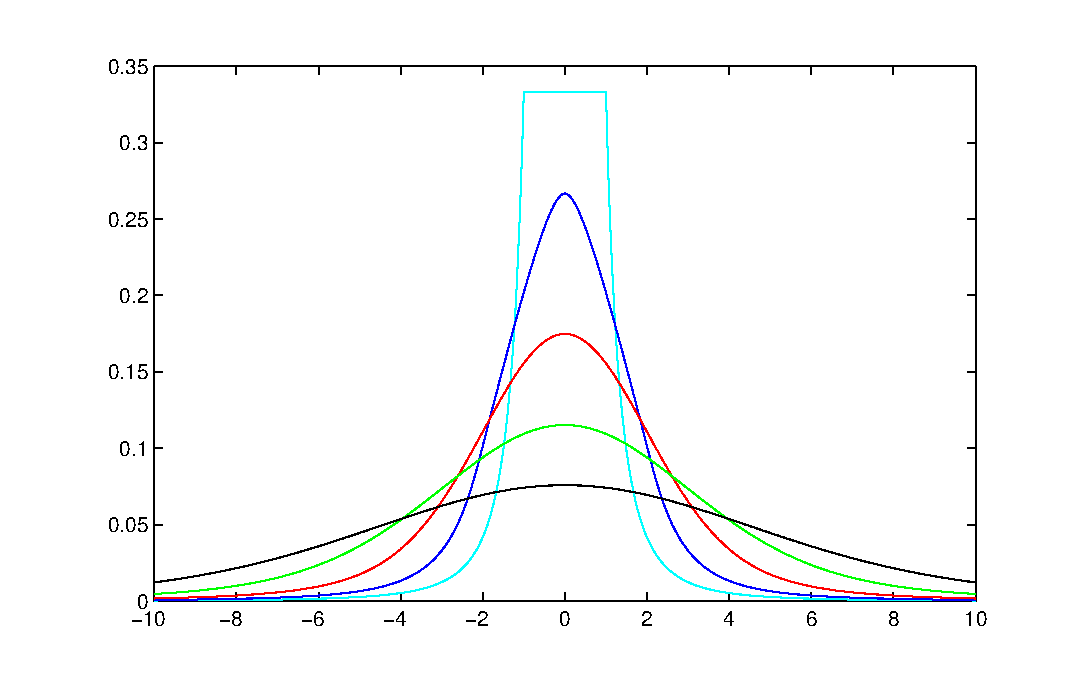
\includegraphics{Statistics/Stable_distribution/x-3_pdf.eps}}
\hspace{-1cm}
\resizebox{.52\textwidth}{!}{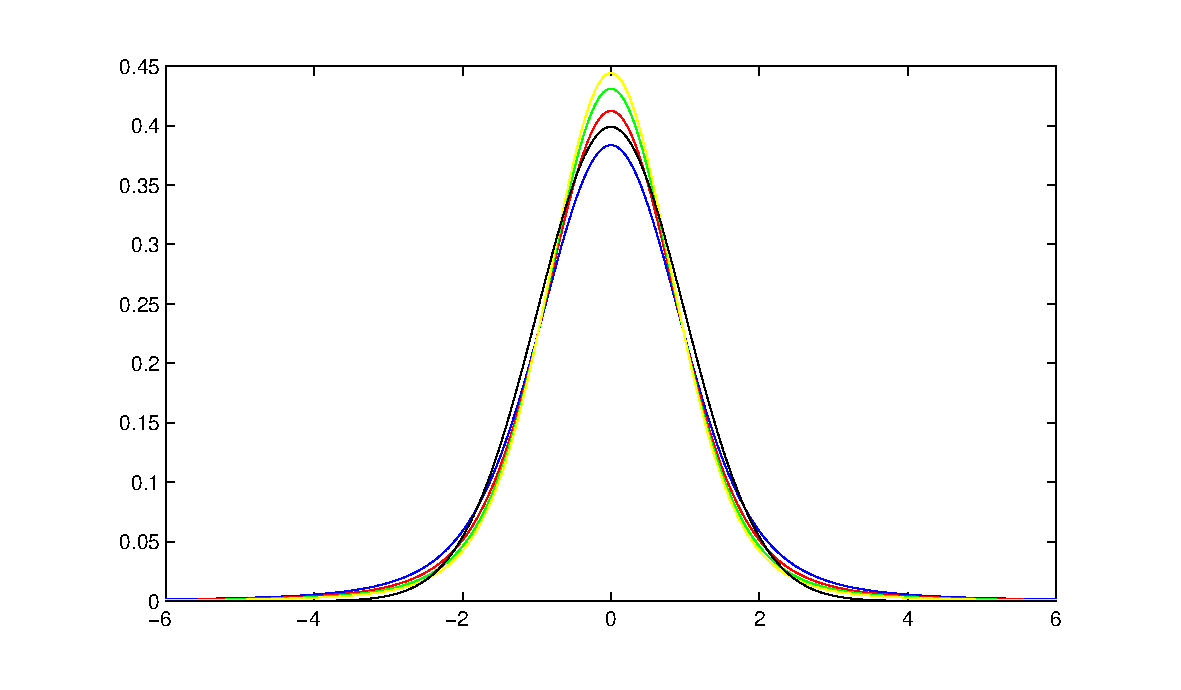
\includegraphics{Statistics/Stable_distribution/x-3_normalized_pdf.eps}}
\end{figure}

It can be proved that it normalized sum converges to a standard normal distribution. 
\end{example}

\begin{example}

Let $X$ be the rv with the density function
\be
f(x) = \left\{\ba{ll}
\frac 12 \abs{x}^{-2} \quad\quad & \abs{x}\geq 1 \\
0  & \abs{x}< 1 
\ea\right.
\ee

The left graph illustrates the convolution $f^{n*}$ of $n=1,2,4,8$ (cyan, blue, red and green, respectively) for this density function. In right graph
we can use $a_n = \frac{n\pi}{2}$, $n=2,4,8$ (blue, red, green). Then the normalized random variable converges to standard Cauchy distribution (black line).

\begin{figure}[thb]
\centering
\resizebox{.49\textwidth}{!}{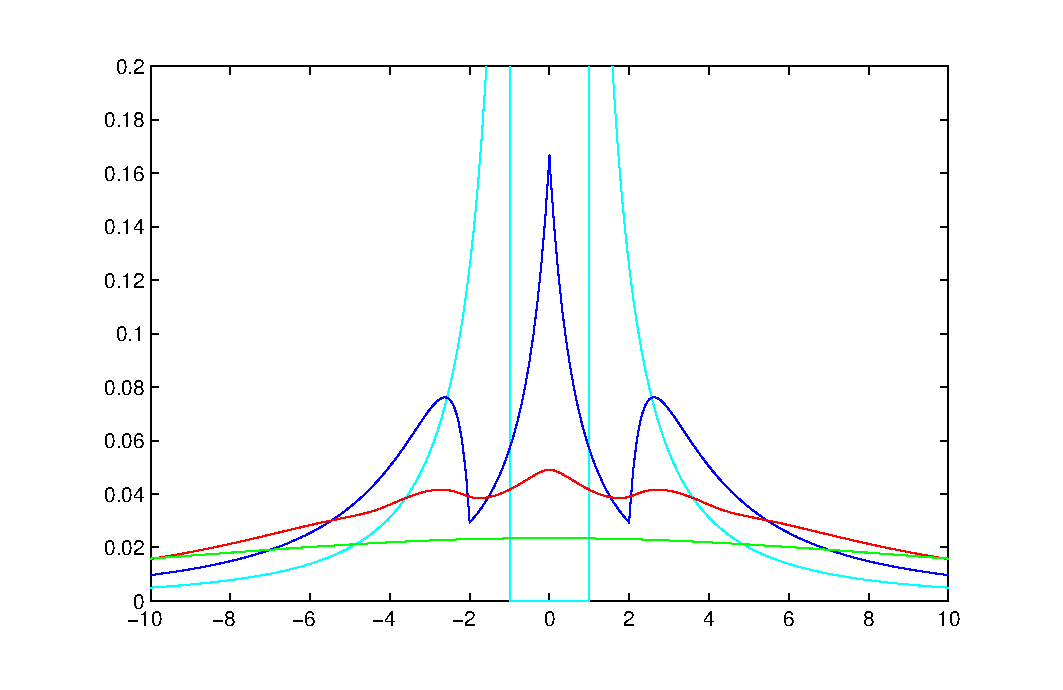
\includegraphics{Statistics/Stable_distribution/x-2_pdf.eps}}
\hspace{-1cm}
\resizebox{.53\textwidth}{!}{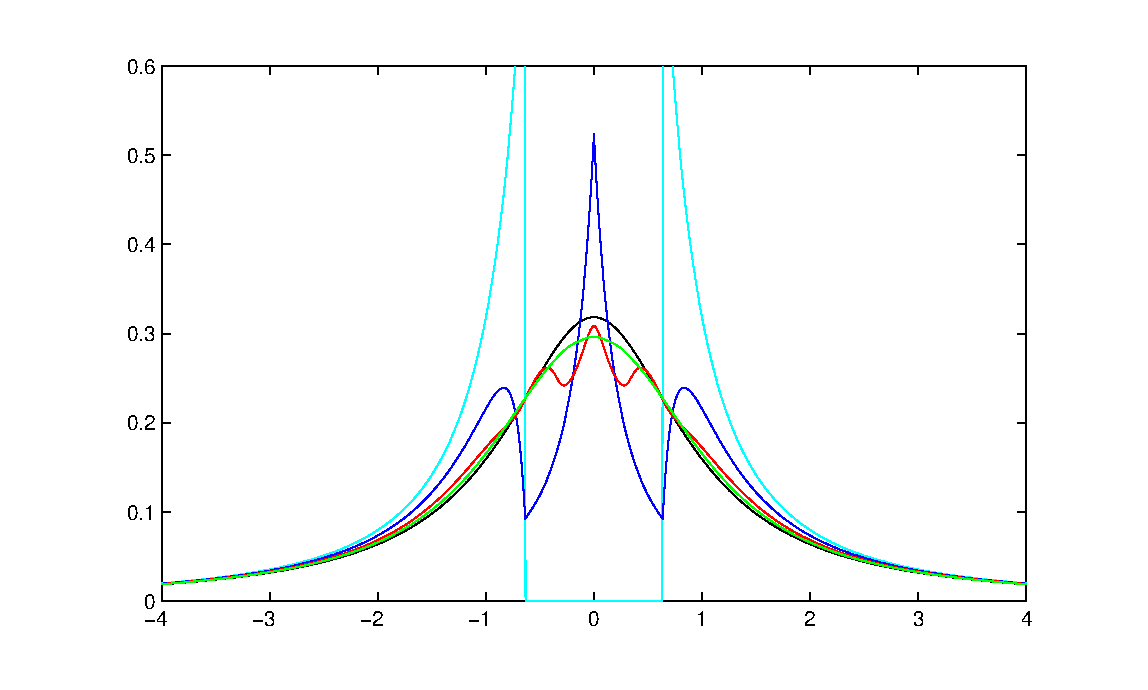
\includegraphics{Statistics/Stable_distribution/x-2_normalized_pdf.eps}}
\end{figure}
\end{example}


